\documentclass[11pt]{article}
\usepackage[cm]{fullpage}
\usepackage{mathtools} %includes amsmath
\usepackage{listings}
\lstset{basicstyle=\ttfamily\small}
\lstset{literate={~} {$\sim$}{1}}
\lstset{showstringspaces=false}
\usepackage{lmodern}
\usepackage{scrextend}
\usepackage{enumitem}
\usepackage{hyperref}
\usepackage{tikz}
\newcommand{\ttf}[1]{{\ttfamily #1}}
\newcommand{\bo}[1]{\ensuremath{\mathbf{#1}}}
\newcommand{\s}{\textbackslash}
\renewcommand{\sp}{\ \ \ \ \ \ \ \ \ \ }
\newcommand{\pt}{\partial}
\newcommand{\fr}[2]{\dfrac{#1}{#2}}
\newcommand{\pr}[1]{\left(#1\right)}
\newcommand{\ord}[1]{\ensuremath{^{(#1)}}}
\newcommand{\ma}[1]{\left(\begin{matrix}#1\end{matrix}\right)}
\newcommand{\pd}[3]{\ensuremath{ \dfrac{ \partial^{#1} #2 }{\partial #3 ^{#1}}}}
\newcommand{\bigo}{\ensuremath{\mathcal{O}}}
\newcommand{\eth}{\ensuremath{^\text{th}}}
\newcommand{\ld}{\ensuremath{\ldots}}
\newcommand{\miniar}[1]{\ensuremath{\begin{smallmatrix}#1\end{smallmatrix}}}

\title{Programming Project 2: Computing the Hessian Matrix Numerically}
\date{}

%beginning of document
\begin{document}
\maketitle

\section*{Description}

The goal of the project is to compute the Hessian (second derivative matrix) of the molecular energy.
That is, if $E(\bo{X})$ represents the energy of an $N$-atom molecule for a set of fixed nuclear coordinates: \footnote{In quantum mechanics, the ``fixed nuclei'' approximation is known as the Born-Oppenheimer approximation.}
\begin{align}
	\bo{X} =&\ \ma{x_1\\y_1\\z_1\\\vdots\\x_N\\y_N\\z_N}\sp
	X_1=x_1,\ X_2=y_1,\ \ldots,\ X_{3N}=z_N
\end{align}
then we wish to determine the matrix $\bo{H}$ with elements
\begin{align}
	\sp H_{AB} = \fr{\pt^2E}{\pt X_A\pt X_B}
\end{align}
which can be explicitly written as
\begin{align}
	\bo{H} =&\ 
	\ma{
		\fr{\pt^2E}{\pt X_1^2}&\fr{\pt^2E}{\pt X_1\pt X_2}&\ldots&\fr{\pt^2E}{\pt X_1\pt X_{3N}}\\
		\fr{\pt^2E}{\pt X_2\pt X_1}&\fr{\pt^2E}{\pt X_2^2}&\ldots&\fr{\pt^2E}{\pt X_2\pt X_{3N}}\\
		\vdots&\vdots&\ddots&\vdots\\
		\fr{\pt^2E}{\pt X_{3N}\pt X_1}&\fr{\pt^2E}{\pt X_{3N}\pt X_2}&\ldots&\fr{\pt^2E}{\pt X_{3N}^2}}
	\label{H}
\end{align}
It is possible, but extremely complicated, to derive analytic expressions for the Hessian matrix of the energy for a specific approximation (Hartree-Fock, MP2, coupled-cluster, etc.).
Another approach, which is applicable to any approximation, is to determine the Hessian at configuration $\bo{X}$ numerically by evaluating the energy for several nuclear configurations $\bo{X}',\bo{X}'',\ldots$ in the vicinity of $\bo{X}$.
Numerical Hessians are necessarily approximate, but can in principle be evaluated to arbitrary precision.

For this project, we will use one of the simplest set of numerical formulas for the Hessian.
Diagonal elements will be given by \footnote{\url{http://en.wikipedia.org/wiki/Finite_difference\#Higher-order_differences}}
\begin{align}
	\fr{\pt^2 E}{\pt X_A^2} \approx&\
	\fr{E(X_A+h)+E(X_A-h)-2E(X_A)}{h^2}
	\label{H-diagonal}
\end{align}
where $h$ represents some small fixed distance, $E(X_A+h)$ represents the energy obtained when the coordinate $X_A$ is moved a distance $h$, and $E(X_A)$ represents the energy $E(\bo{X})$ at the reference configuration, $\bo{X}$.
Off-diagonal elements will be given by \footnote{\url{http://en.wikipedia.org/wiki/Finite_difference\#Finite_difference_in_several_variables}}
\begin{align}
&
	\fr{\pt^2 E}{\pt X_A\pt X_B} \approx
	\tfrac{E(X_A+h,X_B+h)+E(X_A-h,X_B-h)
		-E(X_A+h,X_B)-E(X_A-h,X_B)
		-E(X_A,X_B+h)-E(X_A,X_B-h)+2E(X_A,X_B)}{2h^2}
	\label{H-offdiagonal}
\end{align}
where $E(X_A+h,X_B+h)$ represents the energy when coordinates $X_A$ and $X_B$ are both displaced by $h$, $E(X_A+h,X_B)$ represents the energy when only coordinate $X_A$ is displaced, and $E(X_A,X_B)$ represents the reference energy, $E(\bo{X})$.
This is known as the ``central differences'' approach, because we obtain the derivatives by displacing each coordinate forward and backward relative to its reference value.
Expressions (\ref{H-diagonal}) and (\ref{H-offdiagonal}) may look somewhat complicated, but the derivation is actually quite straightforward and will be included at the end of this hand-out.

This is the procedure we will follow in order to evaluate these expressions:
\begin{enumerate}
	\item read the reference molecular geometry from a file
	\item generate input files to evaluate the energy of the reference configuration and each displaced configuration
	\item run the energy computations described by each input file
	\item read the energy for each configuration from the output file of each computation
	\item plug the energy values into formulas (\ref{H-diagonal}) and (\ref{H-offdiagonal}) in order to construct the Hessian matrix (\ref{H})
\end{enumerate}
This would be a {\it very} tedious and time-consuming procedure by hand.
Programming allows us to put in some extra work early on in exchange for saving boat-loads of time for ourselves in the future.

\newpage
\section{Procedure}
\subsection{Script 1: Read the molecular geometry from \ttf{molecule.xyz}}
\begin{enumerate}[label=\textbf{\arabic*}]
%%%%%%%%%%%%
%%%ITEM 1%%%
%%%%%%%%%%%%
\item {\bf Figure out how to read the number of atoms, the atom labels, and the Cartesian coordinates from \ttf{molecule.xyz}}\\
There are many ways to do this, but the functions \ttf{readline()}, \footnote{\url{https://docs.python.org/2/library/stdtypes.html\#file.readline}} \ttf{readlines()}, \footnote{\url{https://docs.python.org/2/library/stdtypes.html\#file.readlines}} and \ttf{split()} \footnote{\url{https://docs.python.org/2/library/stdtypes.html\#str.split}} provide one simple way.
The first two functions act on file objects, while the \ttf{split()} function acts on a string.
Here is a short example of the sort of thing one can do with the \ttf{split()} function:
\begin{addmargin}{2cm}{}
\begin{lstlisting}[language=python]
>>> string = '1 2 3 4 5  a  b  c  d'
>>> string.split()
['1', '2', '3', '4', '5', 'a', 'b', 'c', 'd']
>>> [ int(x) for x in string.split()[0:5] ]
[1, 2, 3, 4, 5]
\end{lstlisting}
\end{addmargin}
The number of atoms $N$ should be returned as an \ttf{int}, the labels should be returned as an $N$-dimensional list of strings, and the Cartesian coodinates should be returned as a $3N$-dimensional list of \ttf{float}s:
\begin{align}
	[x_1,y_1,z_1,\ldots,x_N,y_N,z_N]
	\label{coords}
\end{align}
corresponding to the configuration vector $\bo{X}$ described above.
%%%%%%%%%%%%
%%%ITEM 2%%%
%%%%%%%%%%%%
\item {\bf Write functions that read the number of atoms, the atom labels, and the Cartesian coordinates from \ttf{molecule.xyz}}\\
Once you figure out how to get the number of atoms, the atom labels, and the Cartesian coordinates from \ttf{molecule.xyz}, you should write functions to return each of these in the form described in the last step.
Here is an example of a function which returns the number of atoms reported in \ttf{molecule.xyz}:
\begin{addmargin}{2cm}{}
\begin{lstlisting}[language=python]
>>> def get_N():
...   return int(open("molecule.xyz").readline())
... 
>>> get_N()
3
\end{lstlisting}
\end{addmargin}


Once these functions are written, you will be able to call them in your other scripts without rewriting the code.
For example, if the script is called \ttf{molecule.py} and contains the \ttf{get\_N()} function above, then you can import that code as follows:
\begin{addmargin}{2cm}{}
\begin{lstlisting}[language=python]
>>> from molecule import *
>>> get_N()
3
\end{lstlisting}
\end{addmargin}
The line \ttf{from molecule import *} is equivalent to pasting the contents of \ttf{molecule.py} into your file or terminal.
Any code contained in that file will be run again, so imported files usually contain only functions and variable definitions.
\end{enumerate}


\subsection{Script 2: Generate input files for displaced geometries.}
Our ultimate goal is to determine second derivatives of the molecular energy with respect to nuclear motion using equations (\ref{H-diagonal}) and (\ref{H-offdiagonal}).
In order to do so, we need to compute the energy at several different points on the potential energy surface:
\begin{enumerate}
	\item singly displaced configurations: for each coordinate $X_A$, we need the energy of the system with that coordinate shifted to $X_A+h$ (forward displacement) as well as the energy of the system with that coordinate shifted to $X_A-h$ (backward displacement), where $h$ is some previously fixed displacement size
	\item doubly displaced configurations: for every unique pair of coordinates $(X_A, X_B), i\neq j$, we need the energy of the system with both coordinates shifted forward, $(X_A+h,X_B+h)$, and the energy of the system with both coordinates shifted backward, $(X_A-h,X_B-h)$
\end{enumerate}
We also need the energy of the reference configuration -- that is, the energy corresponding to the geometry in \ttf{molecule.xyz}.
For this project, you should use a fixed displacement size of $h=0.005~a_0$ (Bohr).

The steps that follow will guide you through the procedure for generating input files for each of these configurations.
\begin{enumerate}[label=\textbf{\arabic*}]
%%%%%%%%%%%%
%%%ITEM 1%%%
%%%%%%%%%%%%
\item {\bf Write a \ttf{make\_input()} function.}\\
This function should take three arguments:
\begin{addmargin}{2cm}{}
\begin{lstlisting}[language=python]
def make_input(dirname,labels,coords):
\end{lstlisting}
\end{addmargin}
The first argument should take a single string containing the name of the directory in which the input file should be placed, the second should take a list of strings containing the atom labels, and the third argument should take a list of \ttf{float}s with coordinates in the form (\ref{coords}).
Using this information, this function should create (or overwrite) a file named ``\ttf{input.dat}'' in the directory ``\ttf{dirname}''.
The input file for the reference configuration should look something like this:
\begin{addmargin}{2cm}{}
\begin{lstlisting}[language=python]
molecule h2o {
units bohr
  O  0.0000000  0.0000000 -0.1345037
  H  0.0000000 -1.6849167  1.0673357
  H  0.0000000  1.6849167  1.0673357
}

set basis cc-pVDZ
energy('scf')
\end{lstlisting}
\end{addmargin}
The \ttf{os} module\footnote{\url{https://docs.python.org/2/library/os.html}} may prove useful for this task -- in particular, functions such as \ttf{makedirs()}\footnote{\url{https://docs.python.org/2/library/os.html\#os.makedirs}} and \ttf{path.exists()} are worth looking at.\footnote{\url{https://docs.python.org/2/library/os.path.html\#os.path.exists}}
To use these functions, you must import the module by adding the line \ttf{import os} near the top of your file.
You will also need the \ttf{write()} function\footnote{\url{https://docs.python.org/2/library/stdtypes.html\#file.write}}, which allows you to write to a file object \ttf{f} as \ttf{f.write(string)}, provided it has been opened in write mode
(\ttf{f=open(filename,"w")}).
You may also want to use string formatting, \footnote{\url{https://docs.python.org/2/library/stdtypes.html\#string-formatting-operations}}
\footnote{\url{http://www.diveintopython.net/native_data_types/formatting_strings.html}} which allows you to have a string with placeholders.
Here is an example of string formatting with placeholders:
\begin{addmargin}{2cm}{}
\begin{lstlisting}[language=python]
>>> for i in range(-3,4):
...   print "%8.3f" % pow(10,i)
... 
   0.001
   0.010
   0.100
   1.000
  10.000
 100.000
1000.000
\end{lstlisting}
\end{addmargin}
(where \ttf{pow(a,b)} is a Python function that returns \ttf{a} to the power of \ttf{b}, $a^b$).
The general syntax is \ttf{string \% (item1,item2,...)}.
This represents a string with placeholders, followed by a ``modulo'' operator \ttf{\%} to indicate that the values for the placeholders are next, followed by a ``tuple'' of values to be filled in.
These can be somewhat tricky to decipher at first, so I recommend getting some help to figure them out.
%%%%%%%%%%%%
%%%ITEM 2%%%
%%%%%%%%%%%%
\item {\bf Devise a naming scheme for the directories.}\\
Each directory will contain one input file in which either one or two coordinates have been displaced by a fixed amount ($h = 0.005~a_0$) forward or backward, as described above.
You should come up with a consistent scheme for naming each directory in a way that identifies which displacement it contains, and use this scheme for the next steps.
%%%%%%%%%%%%
%%%ITEM 3%%%
%%%%%%%%%%%%
\item {\bf Generate the input for the reference configuration.}\\
You should be able to do this using your \ttf{make\_inputs()} function as well as the functions written in the first script.
In my code, this step looks as follows:
\begin{addmargin}{2cm}{}
\begin{lstlisting}[language=python]
from molecule import *
make_input("x0x0_00",get_labels(),get_xyz())
\end{lstlisting}
\end{addmargin}
where the string \ttf{"x0x0\_00"} identifies the directory for the reference configuration in my naming scheme, \ttf{get\_labels()} is my function to return labels (which lives in a script I have called \ttf{molecule.py}), and \ttf{get\_xyz()} is my function to return a vector of coordinates (also in \ttf{molecule.py}).
%%%%%%%%%%%%
%%%ITEM 4%%%
%%%%%%%%%%%%
\item {\bf Generate inputs for single displacements.}\\
As described above, given $N$ atoms with $3$ Cartesian coordinates per atom, we need $3N$ forward displacements and $3N$ backward displacements.
You should be able to use a \ttf{for} loop, combined with your \ttf{make\_inputs()} function and your functions from the first script in order to generate inputs for forward and backward single displacements.
%%%%%%%%%%%%
%%%ITEM 5%%%
%%%%%%%%%%%%
\item {\bf Generate inputs for double displacements.}\\
Given $3N$ coordinates, there are $\fr{3N(3N-1)}{2}$ unique coordinate pairs.
For each pair of coordinates, we need one input file with forward displacements along both coordinates, and one input file with backward displacements along both coordinates.
This step will be very similar to the previous one, except that it requires two nested \ttf{for} loops.
\end{enumerate}
After running your script, you should test a few of the input files by entering the directory and executing \text{Psi4}.  The command to execute \textsc{Psi4} is simply \ttf{psi4}.  The program expects the input file to be named \ttf{input.dat} by default, and prints to a file named \ttf{output.dat} by default.

\subsection{Script 3: Run the input files.}
This script will automate the process of \ttf{cd}-ing into directories and running \ttf{psi4}.
\begin{enumerate}[label=\textbf{\arabic*}]
%%%%%%%%%%%%
%%%ITEM 1%%%
%%%%%%%%%%%%
\item {\bf Write a \ttf{run\_input()} function.}\\
You will once again need the \ttf{os} module.
The \ttf{os.chdir()} function \footnote{\url{https://docs.python.org/2/library/os.html\#os.chdir}} can be used to change directories, and the the \ttf{os.system()} function \footnote{\url{https://docs.python.org/2/library/os.html\#os.system}} can be used to execute a command within a given directory.
While you are troubleshooting your code, the \ttf{os.getcwd()} function may be useful.
This function returns a string representing the path to your current working directory.
%%%%%%%%%%%%
%%%ITEM 2%%%
%%%%%%%%%%%%
\item {\bf Run jobs.}\\
Using your \ttf{run\_input()} function, you can run the job in directory \ttf{dirname} as \ttf{run\_input(dirname)}.
Your script should run jobs for all of the created input files: the reference configuration, the single displacements (one \ttf{for} loop), and the double displacements (two \ttf{for} loops).
\end{enumerate}

\subsection{Script 4: Compute the Hessian matrix using single-point energies}

Equations (\ref{H-diagonal}) and (\ref{H-offdiagonal}) can be expressed more compactly as
\begin{align}
	E_0\ord{2} \approx&\ 
	\fr{E_{+}+E_{-}-2E_0}{h^2} \\
	E_{0,0}\ord{1,1} \approx&\ 
	\fr{E_{+1,+1}+E_{-1,-1}-E_{+1,0}-E_{-1,0}-E_{0,+1}-E_{0,-1}+2E_{0,0}}{2h^2}
\end{align}
where the superscripts represent the order of the derivative with respect to one or two variables, and the subscripts represent the type of displacement (forward, backward, or none) for the same one or two variables.
If you don't like this notation, you can ignore these expressions and look at (\ref{H-diagonal}) and (\ref{H-offdiagonal}).
This script will evaluate these expressions in order to determine
\begin{align*}
	H_{ij} = \fr{\pt^2E}{\pt X_A\pt X_B}
\end{align*}
at the reference configuration $\bo{X}$ in \ttf{molecule.xyz} by reading energies from the output files of the jobs run with the previous script.
\begin{enumerate}[label=\textbf{\arabic*}]
%%%%%%%%%%%%
%%%ITEM 1%%%
%%%%%%%%%%%%
\item {\bf Write a function to return energies.}\\
You should write one or more functions which return the energy corresponding to a particular displacement.
In my code, I have a single function with definition
\begin{addmargin}{2cm}{}
\begin{lstlisting}[language=c++]
def E(i,j,hi,hj):
\end{lstlisting}
\end{addmargin}
where \ttf{i} is the index of one coordinate, \ttf{j} is the index of another coordinate, and \ttf{hi,hj} represent the displacements along \ttf{i} and \ttf{j}, respectively.
That is, \ttf{E(0,0,0,0)} returns the reference energy, \ttf{E(1,0,-1,0)} returns the energy for a single backward displacement along coordinate \ttf{1}, and \ttf{E(7,4,1,1)} returns the energy for a double forward displacement along coordinates \ttf{7} and \ttf{4}.
Another reasonable approach is to have separate functions for single and double displacements -- either one is okay.\\
The task of reading energies from the output files can be achieved using the same set of functions that we used to interpret \ttf{molecule.xyz} in our first script.
My script uses only \ttf{readlines()}.
It is also useful to note that one can obtain sections of strings similar to the way one obtains sections of lists:
\begin{addmargin}{2cm}{}
\begin{lstlisting}[language=c++]
>>> mystring = "abcdef222GFFT"
>>> mystring[0]
'a'
>>> mystring[1:6]
'bcdef'
>>> mystring[7:]
'22GFFT'
\end{lstlisting}
\end{addmargin}
Here is one example of how one might extract a number from a text file:
\begin{addmargin}{2cm}{}
\begin{lstlisting}[language=c++]
>>> mystring = "line1\nline2\nline3\na = 4.0\nline5"
>>> mystring.splitlines()
['line1', 'line2', 'line3', 'a = 4.0', 'line5']
>>> for line in mystring.splitlines():
...   if line[:3] == "a =":
...     print float(line[3:])
... 
4.0
\end{lstlisting}
\end{addmargin}
%%%%%%%%%%%%
%%%ITEM 2%%%
%%%%%%%%%%%%
\item {\bf Initialize the Hessian matrix as a $3N\times3N$ \ttf{list} of \ttf{list}s.}\\
All of the elements should be \ttf{0.0}.  We will fill them in momentarily.
Using two \ttf{for} loops with the \ttf{range()} function, this can be achieved in one line.
%%%%%%%%%%%%
%%%ITEM 3%%%
%%%%%%%%%%%%
\item {\bf Fill in diagonal elements of the Hessian using equation (\ref{H-diagonal}).}\\
Using your function(s) to return energies, this should look very similar to the formula itself.
%%%%%%%%%%%%
%%%ITEM 4%%%
%%%%%%%%%%%%
\item {\bf Fill in off-diagonal elements of the Hessian using equation (\ref{H-offdiagonal}).}\\
This will be similar to the previous step, but will require two \ttf{for} loops instead of one.
%%%%%%%%%%%%
%%%ITEM 5%%%
%%%%%%%%%%%%
\item {\bf Print your Hessian matrix neatly to a file called \ttf{hessian.txt}.}\\
To create/overwrite the file, you can simply \ttf{open()} it in write mode (\ttf{"w"}).
You can write to a file object using the \ttf{write()} function.\footnote{\url{https://docs.python.org/2/library/stdtypes.html\#file.write}}
To make things look neat, you should print each element as a formatted \ttf{float} using placeholders as described above in the instructions for the \ttf{make\_input()} function.
Here is an example of how one might write to a file in Python:
\begin{addmargin}{2cm}{}
\begin{lstlisting}[language=c++]
>>> f = open("newfile","w")
>>> for i in range(18):
...   f.write(" %d" % i)
... 
>>> f.close()
>>> open("newfile").read()
' 0 1 2 3 4 5 6 7 8 9 10 11 12 13 14 15 16 17'
\end{lstlisting}
\end{addmargin}
Once this is done, you should check your answer.
If it doesn't match, you have some debugging to do -- welcome to programming.
If it does match, congratulate yourself! \footnote{Do not expect all of your programs to work without debugging.  Learning to find your mistake is almost as important as learning to program in the first place.}
\end{enumerate}


\newpage
\section{Extra Files}
\subsection{\ttf{molecule.xyz}}
The \ttf{.xyz} format is a standard chemical file format used by visualization programs such as Jmol and cheMVP.
Typically the units for \ttf{.xyz} files are \AA ngstr\"oms (\AA), but the one we are using is in Bohr ($a_0$).
The general structure is as follows:
\begin{addmargin}{2cm}{}
\begin{lstlisting}[language=c++]
N
COMMENT LINE
A1 x1 y1 z1
A2 x2 y2 z2
...
AN xN yN zN
\end{lstlisting}
\end{addmargin}
where the first line contains an integer indicating the number ($N$) of atoms in the molecule, the second line is generally either blank or contains text describing the system, and the final $N$ lines each contain an atomic symbol followed by three numbers indicating the Cartesian coordinates of the atom (hence the extension \ttf{.xyz}).
For this project, we will start with water:
\begin{addmargin}{2cm}{}
\begin{lstlisting}[language=c++]
3
WATER MOLECULE (units Bohr)
O           0.000000000000     0.000000000000    -0.134503695264
H           0.000000000000    -1.684916670000     1.067335684736
H           0.000000000000     1.684916670000     1.067335684736
\end{lstlisting}
\end{addmargin}



\newpage
\section{Derivation of Central Difference 2$^\text{nd}$ Derivative Formulas}

To begin, it should be pointed out that you are likely already familiar with one finite difference formula:
\begin{align*}
	f'(x) = \lim_{h\rightarrow0} \fr{f(x+h)-f(x)}{h}
\end{align*}
This expression is used to define derivatives in Calculus I.
In the language used by applied mathematicians, this would be called a first-order, forward-difference derivative.
That is, a first derivative determined by displacing the function argument by $+h$.
An analogous central-difference derivative expression would be
\begin{align*}
	f'(x) = \lim_{h\rightarrow0} \fr{f(x+h)-f(x-h)}{2h} 
\end{align*}
which involves both forward and backward displacements.

The most straightforward approach to deriving such formulas starts from a Taylor expansion.
\begin{align}
	f(x) 
	=&\
	\sum_{n=0}^\infty \fr{1}{n!}
	\left.\pd{n}{f}{x}\right|_{x=0} x^n
\end{align}
Which, for our purposes, is more conveniently expressed as
\begin{align}
	f(x) =&\
  	f_0 + f_0\ord{1}x + \fr{1}{2!}f_0\ord{2}x^2
  	+ \fr{1}{3!}f_0\ord{3}x^3 + \bigo(x^4)
\end{align}
$f_0\ord{n}$ here simply denotes the value of the $n\eth$ derivative of $f$ at $x=0$.
The last term, $\bigo(x^4)$, describes the magnitude of the error incurred by truncating the Taylor expansion at a particular point -- we are interested in a very small region about $x=0$, so higher powers of $x$ will generally mean better accuracy.

The basic strategy used to derive expressions for the derivatives is to plug in various $x$-values $\{x_k\}$, yielding a series of equations, and then solve for the derivatives in terms of the function values at these points $\{f(X_A)\}$.
Here we will take the ``uniform grid'' approach, in which we use $x$ values with a fixed interval $h$ between them $\{\ld,-2h,-h,0,+h,+2h,\ld\}$.

\subsection{Derivatives of one variable}
To get a first approximation of the first and second derivatives in one variable, we only need three points from our grid $\{-h,0,+h\}$.
Let $f_{\pm k}$ represent $f(\pm kh)$ to keep things a little bit neater.
\begin{align*}
	f_{+1} =&\
	f_0 + f\ord{1}_0 h + \fr{1}{2!}f\ord{2}_0 h^2
	+\bigo(h^3)\\
	f_{-1} =&\
	f_0 - f\ord{1}_0 h + \fr{1}{2!}f\ord{2}_0 h^2
	-\bigo(h^3)
\end{align*}
Hopefully you can see that when we subtract the two equations the even powers of $h$ cancel, which allows us to solve for the first derivative to third order in $h$.
\begin{align*}
	f\ord{1}_0 =&\ \fr{f_{+1}-f_{-1}}{2h} +\bigo(h^3)
\end{align*}
Similarly, adding the two equations cancels even powers which allows us to solve for the second derivative to fourth order in $h$.
\begin{align*}
	f\ord{2}_0 =&\ \fr{f_{+1}+f_{-1}-2f_0}{h^2} +\bigo(h^4)
\end{align*}
You can easily check this on paper.

This formula can be used at $x_0\neq 0$ as well by displacing relative to $x_0$ rather than $0$.
\begin{align*}
	\pr{\fr{\pt^2f}{\pt x^2}}_{x=x_0} = 
	\fr{f(x_0+h)+f(x_0-h)-2f(x_0)}{h^2}+\bigo(h^4)
\end{align*}
Since total derivatives of a one-variable function work just like partial derivatives of one variable in a multivariate function, this generalizes directly to the latter case.

\subsection{Mixed partials}
Since we are ultimately interested in computing second derivatives for a multivariate function, we will also need to find an expression for mixed partial derivatives of the form $\fr{\pt^2f}{\pt x\pt y}$.
The Taylor expansion for a multivariate function is
\begin{align*}
	f(x_1,\ld,x_n) =&\ 
	f_0
	+\sum_{i=1}^n
	\pr{\fr{\pt f}{\pt X_A}}_0X_A
	+\fr{1}{2!}\sum_{i,j=1}^n
	\pr{\fr{\pt^2f}{\pt X_A\pt X_B}}_0X_AX_B
	+\fr{1}{3!}\sum_{i,j,k=1}^n
	\pr{\fr{\pt^3f}{\pt X_A\pt X_B\pt x_k}}_0
	X_AX_Bx_k
	+\ld
\end{align*}
For a bivariate function, we can expand this up to second derivatives (extending the notation used above) as
\begin{align*}
	f(x,y) =
	f_{0,0} + f_{0,0}\ord{1,0}x + f_{0,0}\ord{0,1}y
	+\fr{1}{2!} f_{0,0}\ord{2,0}x^2
	+f_{0,0}\ord{1,1}xy
	+\fr{1}{2!} f_{0,0}\ord{0,2}y^2
	+\ld
\end{align*}
where we are interested in solving for
$f_{0,0}\ord{1,1}\equiv\left.\fr{\pt^2f}{\pt x\pt y}\right|_{x=y=0}$.
The only new points needed for this are 
\begin{align*}
	f_{+1,+1} =&\ 
	f_{0,0} + f\ord{1,0}_{0,0}h+f\ord{0,1}_{0,0}h + 
	\fr{1}{2!}f\ord{2,0}_{0,0}h^2+f\ord{1,1}_{0,0} h^2
	+\fr{1}{2!} f\ord{0,2}_{0,0}h^2
	+\bigo(h^3)
	\\
	f_{-1,-1} =&\ 
	f_{0,0} - f\ord{1,0}_{0,0}h-f\ord{0,1}_{0,0}h + 
	\fr{1}{2!}f\ord{2,0}_{0,0}h^2+f\ord{1,1}_{0,0} h^2
	+\fr{1}{2!} f\ord{0,2}_{0,0}h^2
	-\bigo(h^3)
\end{align*}
By adding together these equations, we obtain
\begin{align*}
	f\ord{1,1}_{0,0} =&\ 
	\fr{f_{+1,+1}+f_{-1,-1}-2f_{0,0} }{2h^2}
	-\fr{f\ord{2,0}_{0,0} + f\ord{0,2}_{0,0}}{2}
	+\bigo(h^4)
\end{align*}
Since $f\ord{2,0}_{0,0}$ and $f\ord{0,2}_{0,0}$ are partial derivatives with respect to a single variable, we can plug in the expression for $f\ord{2}_0$ derived above, giving
\begin{align*}
	f\ord{1,1}_{0,0} =&\ 
	\fr{f_{+1,+1}+f_{-1,-1}
		-f_{+1,0}-f_{-1,0}
		-f_{0,+1}-f_{0,-1}+2f_{0,0}
	}{2h^2}
	+\bigo(h^4)
\end{align*}
Such expressions are sometimes described according to the grid of points used in them.
In this case, we have:
\begin{center}
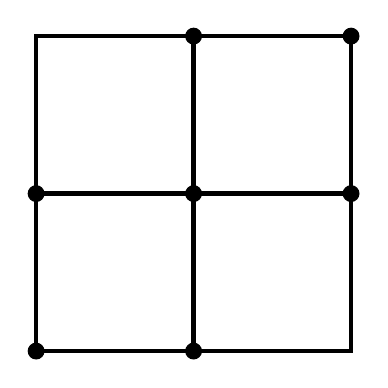
\begin{tikzpicture}[scale=2]
\draw [ultra thick] (-1,-1)--(-1,+1)--(+1,+1)--(+1,-1)--(-1,-1);
\draw [ultra thick] (0,-1)--(0,+1);
\draw [ultra thick] (-1,0)--(+1,0);
\draw[fill] (+1,+1) circle [radius=0.05];
\draw[fill] (+1,0) circle [radius=0.05];
\draw[fill] (0,+1) circle [radius=0.05];
\draw[fill] (0,0) circle [radius=0.05];
\draw[fill] (-1,-1) circle [radius=0.05];
\draw[fill] (-1,0) circle [radius=0.05];
\draw[fill] (0,-1) circle [radius=0.05];
\end{tikzpicture}
\end{center}
where the middle point is the origin and all line segments have length $h$.

As for derivatives of a single variable, the generalization to arbitrary reference values is straightforward:
{\small
\begin{align*}
	&\pr{\fr{\pt^2f}{\pt x\pt y}}_{\miniar{x=x_0\\y=y_0}}\\ & \ \ =
	\fr{f(x_0+h,y_0+h)+f(x_0-h,y_0-h)-f(x_0+h,y_0)-f(x_0-h,y_0)-f(x_0,y_0+h)-f(x_0,y_0-h)+2f(x_0,y_0)}{2h^2} \\ &\sp + \bigo(h^4)
\end{align*} }
and it makes no difference wether or not the function has more than two variables, since these are held constant for partial derivatives.

%end of the document
\end{document}
